\begin{activity} \label{A:3.3.3}  A piece of cardboard that is $10 \times 15$ (each measured in inches) is being made into a box without a top.  To do so,
squares are cut from each corner of the box and the remaining sides are folded up.  If the box needs to be at least 1 inch deep and no more than 3 inches deep, what is the maximum possible volume of the box?  what is the minimum volume?  Justify your answers using calculus.
\ba
	\item Draw a labeled diagram that shows the given information.  What variable should we introduce to represent the choice we make in creating the box?  Label the diagram appropriately with the variable, and write a sentence to state what the variable represents.
	\item Determine a formula for the function $V$ (that depends on the variable in (a)) that tells us the volume of the box.
	\item What is the domain of the function $V$?  That is, what values of $x$ make sense for input?  Are there additional restrictions provided in the problem?
	\item Determine all critical values of the function $V$.
	\item Evaluate $V$ at each of the endpoints of the domain and at any critical values that lie in the domain.
	\item What is the maximum possible volume of the box?  the minimum?
\ea
\end{activity}
\begin{smallhint}
\ba
	\item Consider letting the length of one side of the removed squares be represented by $x$.
	\item Remember that the volume of a box is length $\times$ width $\times$ height.
	\item Read the given information carefully and think about the picture.
	\item Note that since $V$ is a cubic function, $V'$ is quadratic.
	\item Which critical values satisfy $1 \le x \le 3$?
	\item Evaluate the function at appropriate points.
\ea
\end{smallhint}
\begin{bighint}
\ba
	\item Consider letting the length of one side of the removed squares be represented by $x$.  Note, then, that one side of the box will have length $10 - 2x$.
	\item Remember that the volume of a box is length $\times$ width $\times$ height.  Write each of length, width, and height in terms of $x$.
	\item Read the given information carefully and think about the picture.
	\item Note that since $V$ is a cubic function, $V'$ is quadratic, so you can find the critical values exactly.
	\item Which critical values satisfy $1 \le x \le 3$?
	\item Evaluate the function at appropriate points and see which is greatest and which is least.
\ea
\end{bighint}
\begin{activitySolution}
\ba
	\item We let $x$ represent the length of a side of the square that is cut from each corner, so that we have the following picture:
	\begin{center}
	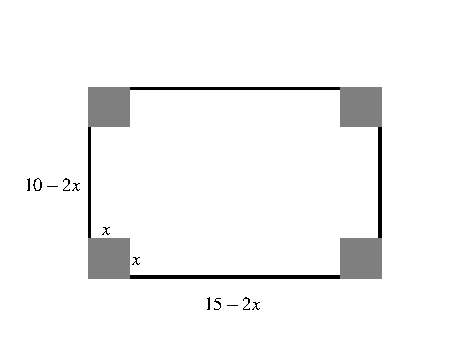
\includegraphics{figures/3_3_Act3Soln.eps}
	\end{center}
	\item Because the box has dimensions $(10-2x) \times (15-2x) \times x$, the volume of the box is given by 
	$$V(x) = x (10-2x) (15-2x) = 4x^3 - 50x^2 + 150x.$$
	\item Clearly the smallest $x$ can be is 0 and the largest $x$ can be is 5, since one side of the cardboard has length 10.  But we're told in the problem to restrict the value of $x$ to $1 \le x \le 3$, so this is the domain we use for $V$, even though $V$ is defined for every real number $x$.
	\item Since $V'(x) = 12x^2 - 100x + 150$, it follows that the critical values (where $V'(x) = 0$) are
	$$x = \frac{25 \pm 5\sqrt{7}}{6} \approx 6.371459426, 1.961873908.$$
	\item Only the latter critical number is in the relevant domain of $V$, and hence we consider
	\begin{itemize}
		\item $V(1.961873908) = 132.0382370$
		\item $V(1) = 104$
		\item $V(3) = 108$
	\end{itemize} 
	\item Hence the absolute maximum possible volume of the box is 132.0382370 and occurs when $x = 1.961873908$, while the absolute minimum is 104, which occurs when $x=1$.
\ea
\end{activitySolution}
\aftera